\section{Signal preprocessing} \label{section:signal-preprocessing}
The vibration signals in a factory environment are inherently full of disturbances. Nearby equipment operation and handling of heavy objects in the surroundings can all contribute to the unwanted chaotic movement in otherwise mostly pure oscillatory motion. In addition, accelerometers suffer from systematic measurement errors in the form of thermal noise, zero-g offset as a result of slight miscalibration, and bias originating from a constant force of gravity. These unavoidable distortions are to some extent suppressible with digital filters. In the preprocessing stage, we consider detrending, noise reduction with adaptive filters, and time synchronous averaging to eliminate the external interference.

\subsection{Detrending}
The oscillatory motion should be centered around the zero level for further manipulation. The constant offset is eliminated simply by subtracting the overall mean from the signal. Moreover high pass DC blocker infinite impulse response (IIR) filter of 1st order can adjust to shifts of the average value over time (Equation~\ref{equ:iir-dc-blocker}). The transition band depends upon the choice of corner frequency $f_{3dB}$ (Fig.~\ref{fig:dc-blocker}).

\myequations{DC blocker IIR filter of 1st order}
\begin{ceqn}\begin{align} \label{equ:iir-dc-blocker}
y_k = (1 - \frac{\omega}{2}) \cdot (x_k  -  x_{k - 1}) + (1 - \omega) \cdot y_{k - 1}; \quad \omega = 2\pi \cdot \frac{f_{3dB}}{f_s}
\end{align}\end{ceqn}

A steeper 3~dB attenuation band can be achieved by increasing the order of the filter. Then the cutoff frequency should be such that filter coefficients are fractions to counteract rounding errors~\cite{tittelbach-helmrich_digital_2021}.

\begin{figure}[h]
	\centering
	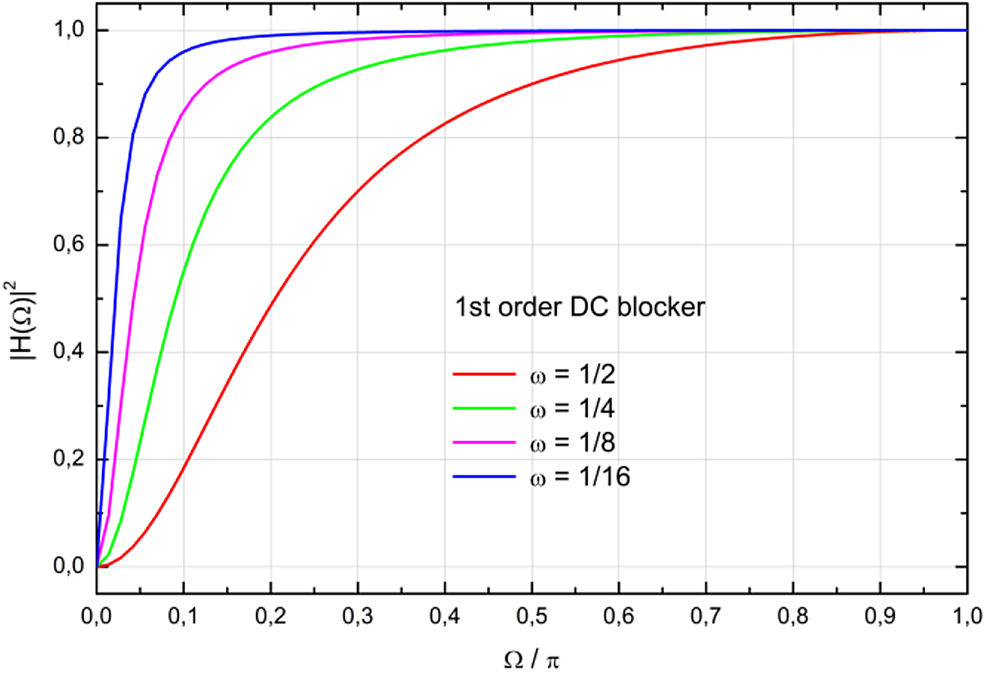
\includegraphics[width=0.7\textwidth]{assets/analysis/iir-1-dc-blocker-band.jpg}
	\caption{Transfer function of 1st order DC blocker filters ~\cite{tittelbach-helmrich_digital_2021}}
	\label{fig:dc-blocker}
\end{figure}

The finite impulse response (FIR) filter is not recommended for DC component removal because of the undesirable ripple effect with the small number of taps. Cascaded-integrator-comb (CIC) filters are proposed as an alternative instead~\cite{lyons_understanding_2011}.

\subsection{Adaptive noise cancellation}
Adaptive noise cancellation (ANC) involves an adaptive filter that self-adjusts coefficients through an update algorithm in response to the reference noise signal.  The objective of this filter is to minimize the mean square error (MSE) cost function in the error signal $e_k$ between signal contaminated with Gaussian noise $d_k$ and filter output $y_k$. Additive noise $n_k$ is assumed to be correlated with noise signal $\mathbf{X_k}$~\cite{diniz_adaptive_2020}.

Wiener-Hopf equations solve the optimal gradient of the MSE function and provide us with FIR filter coefficient vector $\mathbf{W_k}$.  The least mean squares (LMS) algorithm recursively approximates this analytical solution with the method of steepest descent (Equation~\ref{equ:lms-adaptive-filter})~\cite{diniz_adaptive_2020}. The multiple parameters are to be considered in the evaluation of filter performance: convergence rate, estimated error, and signal-to-noise ratio (SNR).

\myequations{Adaptive noise filtering LMS update formula}
\begin{ceqn}\begin{align} \label{equ:lms-adaptive-filter}
\mathbf{W}_{k+1} = \mathbf{W}_{k} + 2 \mu \mathbf{X}_{k}  e_k
\end{align}\end{ceqn}

The convergence stability is affected by step size $\mu$ which is bounded from above with the inverse of the maximal eigenvalue of input covariance matrix $\lambda_{max}$. The normalized least mean squares (NLMS) can handle input of varying scales  (Equation~\ref{equ:nlms-adaptive-filter}).

\myequations{Adaptive noise filtering NLMS update formula}
\begin{ceqn}\begin{align} \label{equ:nlms-adaptive-filter}
\mathbf{W}_{k+1} = \mathbf{W}_{k} + \frac{\mu}{\lVert\mathbf{X}_{k}\rVert^2} \mathbf{X}_{k}  e_k
\end{align}\end{ceqn}

\begin{figure}[h]
	\centering
	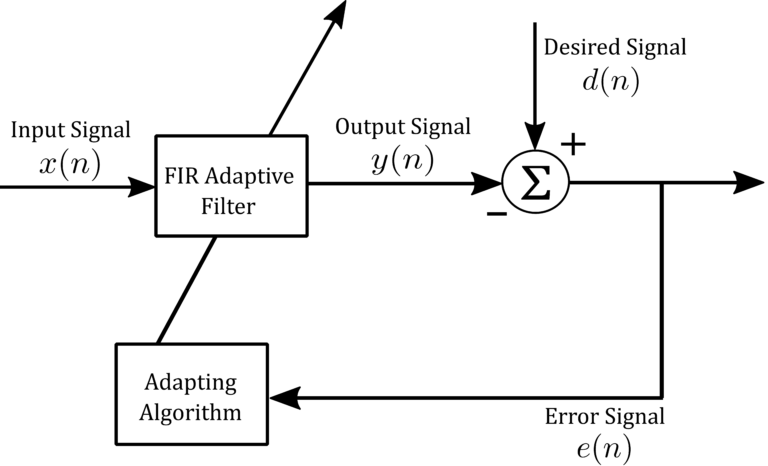
\includegraphics[width=0.8\textwidth]{assets/analysis/adaptive-filter.png}
	\caption{Adaptive noise cancellation filter diagram}
	\label{fig:adaptive-filter}
\end{figure}
\bigbreak

\subsection{Time synchronous averaging}
Time synchronous averaging (TSA) diminishes the impact of vibration sources unrelated to the rotational frequency and its harmonics. TSA averages time-domain waveform over $N$ points and aligns it to a synchronization pulse with period $T$ (Equation~\ref{equ:tsa-average}). 

\myequations{Time synchronous averaging}
\begin{ceqn}\begin{align}
x_{TSA} = \frac{1}{N} \sum_{n = 0}^{N - 1}{x(t + nT)}
\label{equ:tsa-average}
\end{align}\end{ceqn} 

This technique has been successfully applied to the gearbox and bearing fault diagnosis~\cite{davies_handbook_2012,nandi_condition_2019}.

\section{Feature extraction} \label{section:feature-extraction}
After preprocessing raw numerical vectors are merely low-level descriptors of the underlying physical phenomena. At first, these incomprehensible sequences of numbers are reduced to summary attributes called features in the process of feature extraction or feature discovery. Features can be hand-crafted (as is our case), learned implicitly within the model representation, or explicitly from an optimization problem solution. 

Predictive maintenance has ideal prerequisites for the application of feature engineering because the signal is usually pseudo-stationary, and the trend monitoring variables come out of extensive domain expertise in mechanics. The advantages of add-in extraction effort, as opposed to processing samples unmodified, are to gain better classification precision, reduce computational burden and storage capacity downstream with dimensionality reduction~\cite{johnson_feature_2019}. 

It is important to note that the design of features is not a standalone step in the machine learning pipeline but it should be performed iteratively to improve the target model. Signal features are computed in the time, frequency, and time-frequency domain~\cite{brito_fault_2021}.

\subsection{Temporal domain features}
The most widely found features in the literature are rudimentary statistical measures of the central moment: mean, variance, standard deviation, skewness, and kurtosis~(Tab.~\ref{tab:td-features}). Statistics can be calculated in any domain, but the mean value should not to be used in detrended data. The vibration severity metrics out of technical standards are also highly regarded. The characteristics of amplitude include root mean square, peak-to-peak distance, and maximum~\cite{mostafavi_novel_2021}.

The other significant time-domain attributes are derived as ratios of previous simpler ones. These ratios are crest factor, margin factor, impulse factor, and shape factor~(Tab.~\ref{tab:td-features})~\cite{nandi_condition_2019}. Many articles have been successful in bearing fault detection out of transients in impulsive signals with kurtosis, crest factor, and margin indicators \cite{brito_fault_2021}. It is also suggested that the shape factor can signify unbalance and misalignment faults~\cite{nandi_condition_2019}.

\begin{table}[h]
\centering
\renewcommand{\arraystretch}{2}
\begin{adjustbox}{width=\columnwidth,center}
\begin{tabular}{|l|l|l|l|}
\hline
\textbf{Feature}            & \textbf{Equation}                                                                    & \textbf{Feature}        & \textbf{Equation}                                                                                                  \\ \hline
\textit{Standard deviation} & $ X_\sigma = \sqrt{\frac{1}{N}\sum_{i = 1}^{N}{\left(x_i - \bar{x}\right)^2}} $        & \textit{Crest factor}   & $ X_{cf} = \frac{max(|x_i|)}{X_{rms}} $                       \\ \hline
\textit{Skewness}           & $ X_{sv} = \frac{1}{N}\sum_{i = 1}^{N}{\left(\frac{x_i - \bar{x}}{\sigma}\right)^3}$ & \textit{Margin factor}  & $ X_{mf} = \frac{max(|x_i|)}{\left( \frac{1}{N} \sum_{i=1}^{N}{\sqrt{|x_i|}} \right)^2} $                          \\ \hline
\textit{Kurtosis}           & $ X_{kv} = \frac{1}{N}\sum_{i = 1}^{N}{\left(\frac{x_i - \bar{x}}{\sigma}\right)^4}$ & \textit{Impulse factor} & $ X_{if} = \frac{max(|x_i|)}{\frac{1}{N} \sum_{i=1}^{N}{|x_i|}} $                                                  \\ \hline
\textit{Root mean square}   & $ X_{rms} = \sqrt{\frac{1}{N}\sum_{i = 1}^{N}{x_i^2}} $             & \textit{Shape factor}   & $ X_{sf} = \frac{X_{rms}}{\frac{1}{N} \sum_{i=1}^{N}{|x_i|}}$ \\ \hline
\textit{Peak-to-peak}       & $ X_{ppv} = \max(x_i) - \min(x_i) $                                                  & \textit{Maximum}        & $ X_{max} = \max(|x_i|) $                                                                                          \\ \hline
\end{tabular}
\end{adjustbox}
\caption{Temporal domain features}
\label{tab:td-features}
\end{table}

\subsection{Spectral domain features}
The mechanical faults present themselves as oscillatory patterns which are combinations of frequencies with various amplitudes. The Fourier transform is one of the most prominent strategies in power spectral density estimation. Experts on vibrodiagnostics utilize it as a primary signal processing technique for data analysis as it is recommended in ISO 13373-2 standard~\cite{noauthor_iso_2016_2}. 

The inherent symmetries in the Fourier matrix made it possible to implement the Fast Fourier transform (FFT) algorithm with time complexity $O(n \log n)$. The drawback of the plain spectral analysis is the lack of resolution for events that occurred at distant time instants, and so their spectral components might adversely blend in together. 

\begin{table}[ht]
\renewcommand{\arraystretch}{2}
\centering
\begin{adjustbox}{width=\columnwidth,center}
\begin{tabular}{|l|l|}
\hline
\textbf{Feature}           & \textbf{Equation}                                                                                                  \\ \hline
\textit{Spectral centroid} & $ X_{fc} = \frac{\sum_{i = 0}^{N - 1}{f_i \cdot a(f_i)}}{\sum_{i = 0}^{N - 1}{a(f_i)}}$                   \\ \hline 
\textit{Energy}            & $ E(N) = \sum_{i = 1}^{N} a^2(t) $                                                                    \\ \hline \textit{Energy ratio}                & $E_r = E_i \;/\; \sum_{i = 1}^{N}{E_i} $                                                        \\ \hline
\textit{Spectral roll-on} & $ E(f_c) = 0.05 \cdot E(f_s / 2) $ \\ \hline                    
\textit{Spectral roll-off} & $ E(f_c) = 0.95 \cdot E(f_s / 2) $                                                   \\ \hline
\textit{Spectral flux}     & $X_{\mathrm{flux}} = 1 - \mathrm{corr}(A_{t-1}, A_t)$ \\ \hline 
\textit{Noisiness}                   & $X_{noise} = \mathrm{SNR}(X) = \mu \;/\; \sigma $                             \\ \hline
\textit{Shannon entropy}      & $H(X) = - \sum_{i} P(X = x_i) \cdot \ln(P(X = x_i)) $                                                  \\ \hline
\textit{Spectral negentropy}      & $\Delta I_E(f, \Delta f) = \sum_{k = 0}^{N - 1}{\frac{E(k, f, \Delta f)^2}{\frac{1}{N} \sum_{k=0}^{N-1} E(k, f, \Delta f)^2}} \cdot \ln\left(\frac{E(k, f, \Delta f)^2}{\frac{1}{N} \sum_{k=0}^{N-1} E(k, f, \Delta f)^2}\right)$                                                \\ \hline
\end{tabular}
\end{adjustbox}
\caption{Frequency domain features}
\label{tab:fd-features}
\end{table}

In the spectral domain, we can obtain usual statistical properties of the distribution being spectral centroid, skew and kurtosis. Additionaly spectral roll-on and roll-off, fundamental frequency, spectral flux, signal to noise ratio (noisiness), energy in frequency bands, and energy ratio are extracted (Tab.~\ref{tab:fd-features})~\cite{peeters_large_2004}. 

In geometric terms, the spectral centroid represents the barycenter of the frequency magnitude plot. Spectral roll-off gives a notion about the spectral distribution because it identifies the frequency $f_c$ below which 95\% of the signal energy is contained. Complementary, the roll-on frequency is chosen so that 5\% of the signal energy is below this value. According to the definition, spectral flux is normalized cross-correlation between two successive amplitude spectra, a value of one means spectra are the most dissimilar.

``Negentropy measures the inclination of a system to increase its level of organization''~\cite{avoci_spectral_2020}. The larger \emph{spectral negentropy} suggests more fault-induced impulses. $E(k, f, \Delta f)$ denotes the squared envelope spectrum (SES) which is an envelope in the Fourier domain: $\mathcal{F}\{ |y(k, f, \Delta f)|^2 \}$.

If a single principal frequency exists, it can be determined with maximum likelihood estimation. Such frequency would explain the signal spectrum the best~\cite{peeters_large_2004}.  The frequency spectrum is a discrete set of amplitudes where peaks have to be reliably identified to create representative attributes.

The essential peak-finding approaches are based either on magnitude or gradient. All found extrema are commonly filtered with the magnitude of prominences and the widths at half prominence. In the magnitude-based method, middle point $x_i$ is compared to neighboring two points and the peak is then: $x_{i-1} < x_i > x_{i+1}$. The gradient-based method evaluates the first derivative at the point which is equal to zero in case the point is a local maximum, local minimum, or inflection point~\cite{adikaram_non-parametric_2016}.

A substantial improvement is a robust non-parametric peak identification named \emph{MMS} based on the sum of terms in an arithmetic progression based on maximum, minimum, and sum. MMS max-min finder in the elementary form processes points in the window of length 3, it advances one point and deems its middle point as a local extremum if it satisfies equalities below. Equation~\ref{equ:mms-maxima} is for the hill and Equation~\ref{equ:mms-minima} is for the valley. The filtration techniques are incorporated in the adaptations of the MMS algorithm: MMS-WBF, MMS-SG, MMS-LH~\cite{adikaram_non-parametric_2016}.

\myequations{MMS algorithm: Local maxima identification equality}
\begin{ceqn}\begin{align}
\frac{a_{max} - a_{min}}{S_3 - a_{min} \cdot 3} = \frac{a_{mid} - a_{min}}{S_3 - a_{min} \cdot 3}
\label{equ:mms-maxima}
\end{align}\end{ceqn}

\myequations{MMS algorithm: Local minima identification equality}
\begin{ceqn}\begin{align}
\frac{a_{max} - a_{min}}{a_{max} \cdot 3 - S_3} = \frac{a_{max} - a_{mid}}{a_{max} \cdot 3 - S_3}
\label{equ:mms-minima}
 \end{align}\end{ceqn}

Multiple harmonic series and the sidebands can be separated into a discrete set of frequency components, each with central frequency, uncertainty, and amplitude $C_i(v_i, \Delta v_i, A_i)$ by an exhaustive search algorithm. Harmonic family identification is a non-trivial problem because of the spectrum estimation errors. The criterion is proposed to select harmonic at the minimal distance from the true fundamental frequency multiple~(Equation~\ref{equ:harmonic-search}). Two series with the same fundamental frequency are merged and thought of as a modulation series~\cite{gerber_identification_2013}.

\myequations{Harmonic series search criterion}
\begin{ceqn}\begin{align}
v_i^{(r)} = \frac{v_j}{\min{|v_j - r \cdot v_i|}}
\label{equ:harmonic-search}
\end{align}\end{ceqn}

\subsection{Time-frequency domain features}
The \textbf{Short-time Fourier transform} (STFT) splits the time-domain signal to an equal-length intervals. Individual chunks have 50\% overlap and are multiplied with weights of window function to balance scalloping loss and spectral leakage due to Fourier transform periodicity assumption. Traditionally, the Hann window is commonly used instead of rectangular window~\cite{ziaran_technicka_2013,noauthor_iso_2016_2}.

In the time-frequency domain, the same features can be derived as in the frequency domain, but in addition, the attributes are time-localized in this way. The STFT has a considerable flaw for implementation in a self-adaptable system and that is fixed resolution. The optimal window size has to be set beforehand or chosen after performing multiple transformations on chunks out of the range of lengths. Welch's methods averages multiple consecutive blocks to better estimate the spectrum. We have already researched the suitability of STFT for online detection of constant frequencies~\cite{hajek_iot_2022}.

The alternative to isolating weak impacts with high time resolution is a \textbf{Teager-Kaiser energy operator} (TKEO) (Equation~ \ref{equ:tkeo-operator}). It is a tool for envelope analysis to demodulate characteristic AM-FM signal present during bearing faults. Energy operator output can be utilized as a standalone feature attribute.

\myequations{Teager–Kaiser energy operator}
\begin{ceqn}\begin{align}
\psi[x(n)] = [x(n)]^2 - x(n - 1)x(n + 1)
\label{equ:tkeo-operator}
\end{align}\end{ceqn}

Improved TKEO is necessary to prevent analysis from suffering from the noisy source. The key idea is to perform TKEO after signal decomposition into narrow-band components with different center frequencies. The extracted modes are reconstructed with weights assigned based on their correlations to the original signal~\cite{shi_application_2022}.

Time-frequency spectrum modification preserving localization of abrupt wide-band spikes at time $t_0$ and simultaneously reducing energy smear over the larger region is a goal of \textbf{Transient-extracting transform} (TET). Post-processing of STFT window $G(t,\omega)$ involves multiplication of the spectrum with the Transient extracting operator (TEO). This operator is expressed in the form of a Dirac delta function $\delta(t)$ (Equation~\ref{equ:tet-transform}).

\myequations{Transient-extracting transform}
\begin{ceqn}\begin{align}
\mathrm{Te}(t,\omega) = G(t,\omega) \cdot  \delta(t - t_0)
\label{equ:tet-transform}
\end{align}\end{ceqn}

TET representation retains non-zero coefficients where the absolute value of the ratio between two STFTs $G^{tg}[n, k]\;/\;G[n, k]$ is less than half the sampling interval $T$. These two transforms use distinct windows $g[n]$ and $n \cdot g[n]$. Decomposition of signal with TET is proved to produce significantly larger kurtosis (around 38 in TET, 4 in other methods) and hence better discriminate the transient fault~\cite{yu_concentrated_2020}.

\subsection{Wavelet domain features}
The bands for lower frequencies should be longer in duration than for higher frequencies. The \textbf{Wavelet transform} (WT) possesses such multi-scale discrimination property effectively increasing resolution in time-frequency plain. Wavelet basis functions are constructed for that purpose (Equation~\ref{equ:mother-wavelet}). There are several wavelet families, for example, Haar, Daubechies, Coiflets, Symlets, Morlet, and Meyer~\cite{nandi_condition_2019}.

\myequations{Mother wavelet function}
\begin{ceqn}\begin{align}
\psi_{s, \tau} = \frac{1}{\sqrt{s}}\psi\left(\frac{t - \tau}{s}\right)
\label{equ:mother-wavelet}
\end{align}\end{ceqn}

\textbf{Continuous Wavelet transform} (CWT)~(Equation~\ref{equ:cwt-transform}) is performed by scaling and translating the mother wavelet $\psi$ picked out of the appropriate family~\cite{nandi_condition_2019}. The scale factor is denoted with~$s$ and time position with~$\tau$. The choice of wavelet type is data-driven because distinct wavelet shapes have an impact on the response and ultimately contribute to filter length. The decision lies between recognition abilities for impulse-like signals or the inclusion of wider surrounding space.

\myequations{Continuous Wavelet transform}
\begin{ceqn}\begin{align}
W_{x(t)}(s, \tau) = \frac{1}{\sqrt{s}}\int x(t) \cdot \psi^*\left(\frac{t - \tau}{s}\right)\;\mathrm{dt}
\label{equ:cwt-transform}
\end{align}\end{ceqn}

The CWT is computationally intensive when a highly detailed scale resolution is required because each wavelet scale convolves with the entire signal. The fCWT algorithm allows 100 times higher spectral resolution then previous implementation at the same speed. It increases performance 122 times compared to Wavelib and 34 times in comparison with PyWavelets~\cite{arts_fast_2022}. 

The fast CWT algorithm reaches compelling improvement by applying Parseval's theorem to the wavelet transform formula that removes the dependence on the time offset parameter~\cite{arts_fast_2022}. The convolution takes place with the mother wavelet in the Fourier base. Then, inverse FFT produces the coefficients for individual scales.

\textbf{Synchrosqueezing Wavelet transform} (SST) is a modification of CWT attempting to sharpen the representation of frequency components by coefficient reassignments from around the central frequencies towards the middle of the bands. The justification for these reallocations is rooted in the signal approximation as amplitude-modulated oscillating modes with additive noise $\eta(t)$ (Equation~\ref{equ:sst-transform})~\cite{herrera_applications_2014}.

\myequations{Representation of components for Synchrosqueezing Wavelet transform}
\begin{ceqn}\begin{align}
s(t) = \sum_{k=1}^{K} A_k(t)\cos(\theta_k(t)) + \eta(t)
\label{equ:sst-transform}
\end{align}\end{ceqn}

The components are defined by their instantaneous amplitudes $A_k(t)$ and instantaneous phases $\theta_k(t)$. The energy spread to adjacent bins can be effectively squeezed only in regions with constant phase and large enough component separation. Despite the promising properties of this transform, white noise causes severe interference in the resulting time-frequency map.

The spectrograms to illustrate the difference in the ability of Fourier transform, continuous Wavelet transform, and their modifications to pick up underlying patterns in bearing faults are shown in the Fig.~\ref{fig:transforms}.

\begin{figure}[ht]
    \centering
    \begin{subfigure}[b]{0.49\textwidth}
        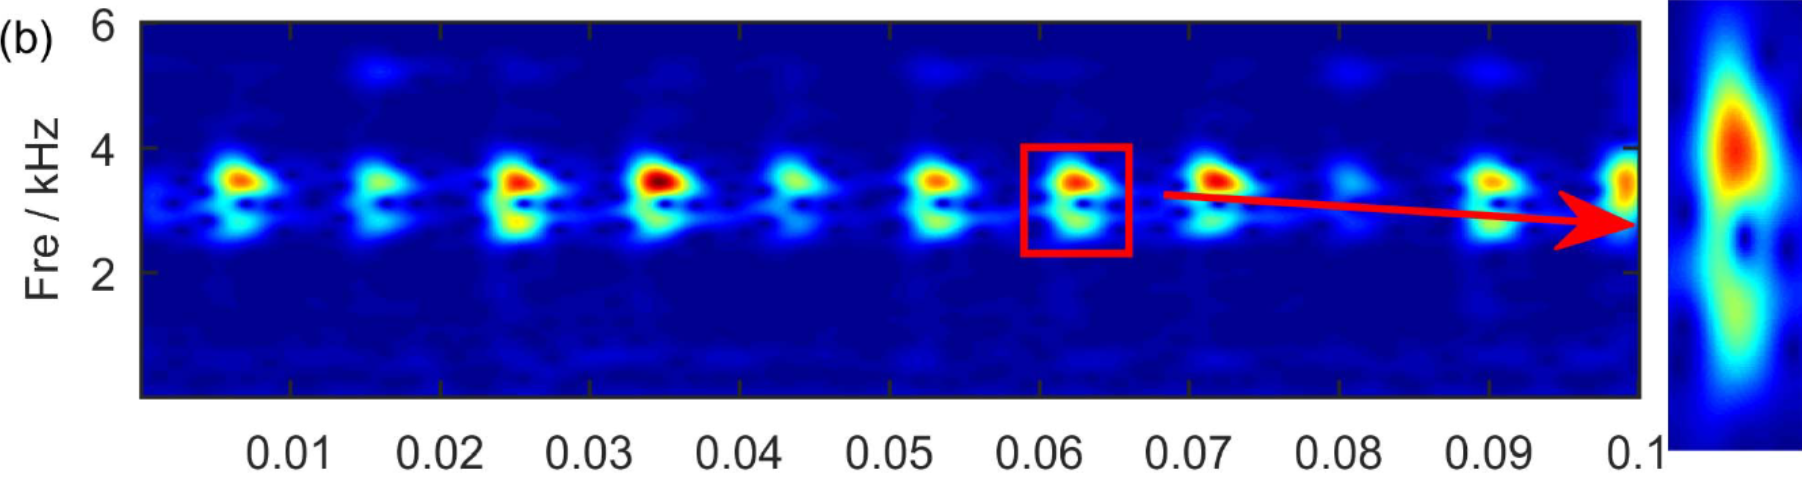
\includegraphics[width=\textwidth]{assets/analysis/stft-spectrogram-sample.png}
        \caption{STFT \& Gaussian window}
    \end{subfigure}
    \hfill
    \begin{subfigure}[b]{0.49\textwidth}
        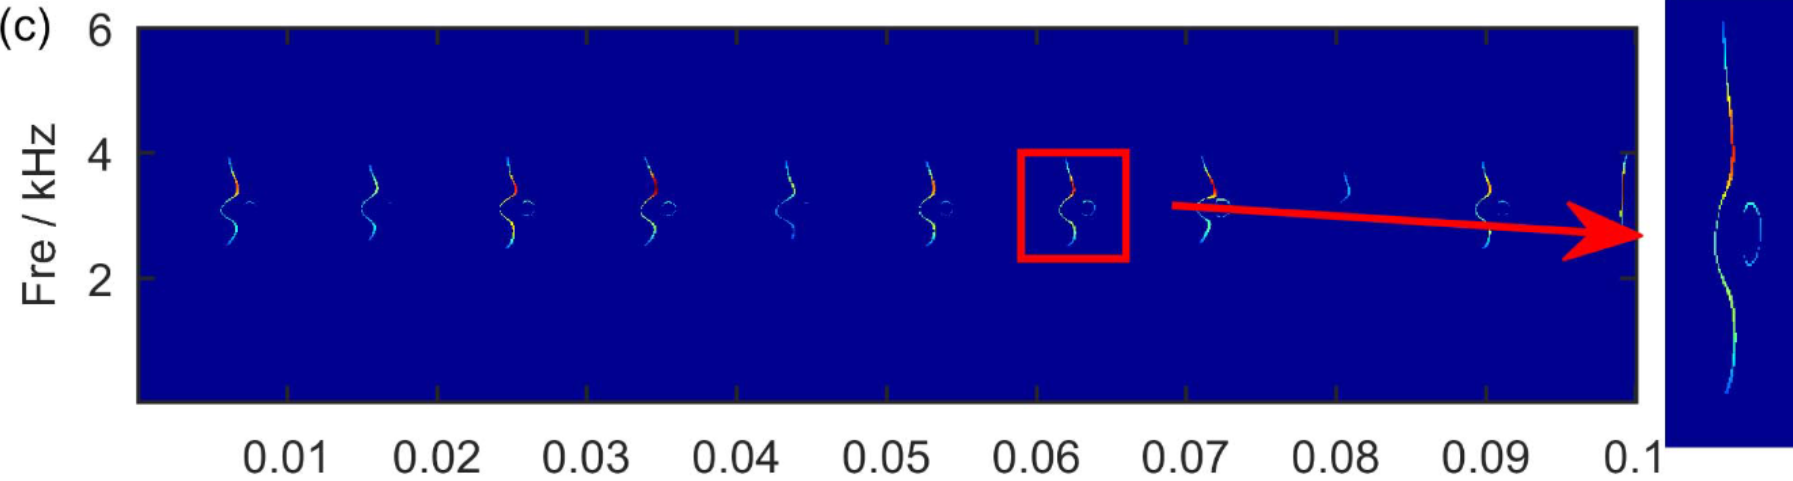
\includegraphics[width=\textwidth]{assets/analysis/tet-spectrogram-sample.png}
        \caption{TET}
    \end{subfigure}
    \hfill
    \begin{subfigure}[b]{0.49\textwidth}
        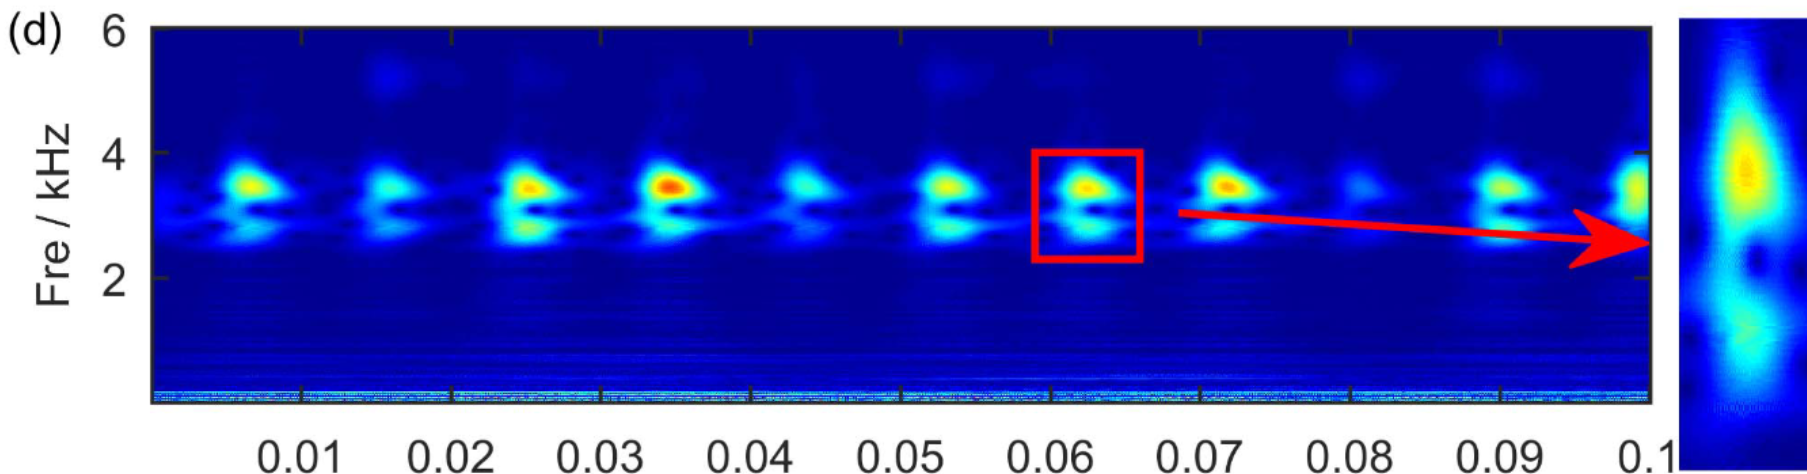
\includegraphics[width=\textwidth]{assets/analysis/wt-spectrogram-sample.png}
        \caption{CWT \& Morlet wavelet}
    \end{subfigure}
    \hfill
    \begin{subfigure}[b]{0.49\textwidth}
        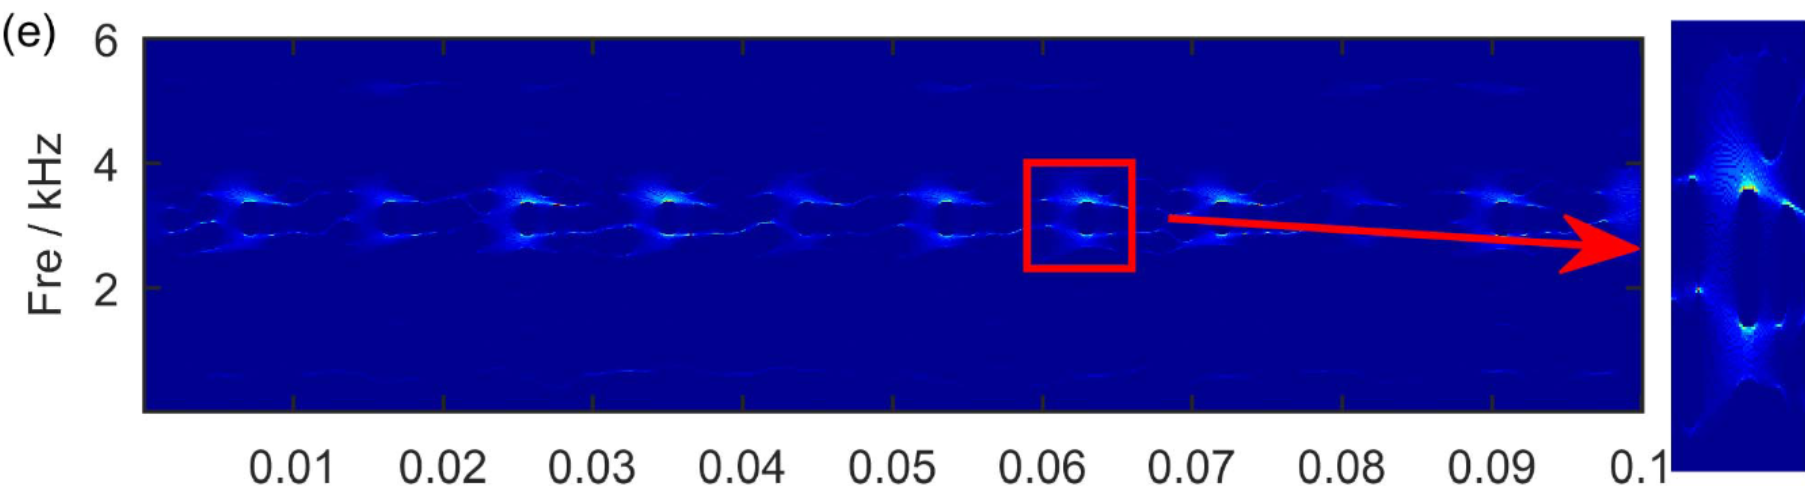
\includegraphics[width=\textwidth]{assets/analysis/sst-spectrogram-sample.png}
        \caption{SST}
    \end{subfigure}
    \caption{Comparison of time-frequency transform spectrograms~\cite{yu_concentrated_2020}}
    \label{fig:transforms}
\end{figure}

The dyadic filter bank is another signal decomposition technique that generates subbands on multiple granularity levels. The practical realization of the multi-scale description is \textbf{Discrete Wavelet Transform} (DWT). The DWT behaves as a quadrature mirror filter and splits waveform using a wavelet filter to detail coefficients (D1) and approximation coefficients (A1) (Fig.~\ref{fig:dwt-filter-bank})~\cite{nandi_condition_2019}. Low-pass filter $h(k)$ creates approximation coefficients further decomposed in the successive levels. Detail coefficients represent the result of the high-pass filter $g(k) = (-1)^k h(1 - k)$ after decimation by the factor of 2. 

The maximum depth of the decomposition tree is $\log_2{n}$ where $n$ is the number of input samples. Energy, energy ratio, and entropy are prevalent features that succinctly encode the wavelet coefficients. Otherwise, the additional extracted levels raise the total number of data dimensions.

In washing machine status classification, the discrete wavelet transform with Daubechies wavelet (db4) and fifth-level decomposition provided features combined from approximation (cA5) and detail coefficients (cD1, \dots, cD5). Washing machines belonged to three categories: no fault, electric motor clamping screws problem, and a loose or broken counterweight. Extracted measures were sample mean and sample variances over autocorrelation functions of coefficients (AcD$n$) and smoothed coefficients cD1, cD2 by moving average filter~\cite{goumas_classification_2002}.

\textbf{Wavelet Packet Decomposition} (WPD) applies filters to split detail coefficients identically as approximation ones (Fig.~\ref{fig:wpd-filter-bank}) thus increasing the resolution in the high-frequency bands and providing uniform spectrum partitioning. 

\myequations{Wavelet packet coefficient}
\begin{ceqn}\begin{align}
 w_{j,n,k} = \langle f, W_{j,k}^n\rangle = \langle f, 2^{j/2} W^n (2^jt-k) \rangle
\label{equ:wavelet-packet-coefficient}
\end{align}\end{ceqn}

Each wavelet packet coefficient $w_{j,n,k}$ captures subband frequency content around time instant $2^j k$ (Equation~\ref{equ:wavelet-packet-coefficient})~\cite{yen_wavelet_2000}. This measure is an inner product of the source and scaled wavelet packet function. The aforementioned feature extraction established in DWT can be applied, for example calculation of the wavelet packet node energy.

\begin{figure}[ht]
    \centering
    \begin{subfigure}[b]{0.49\textwidth}
        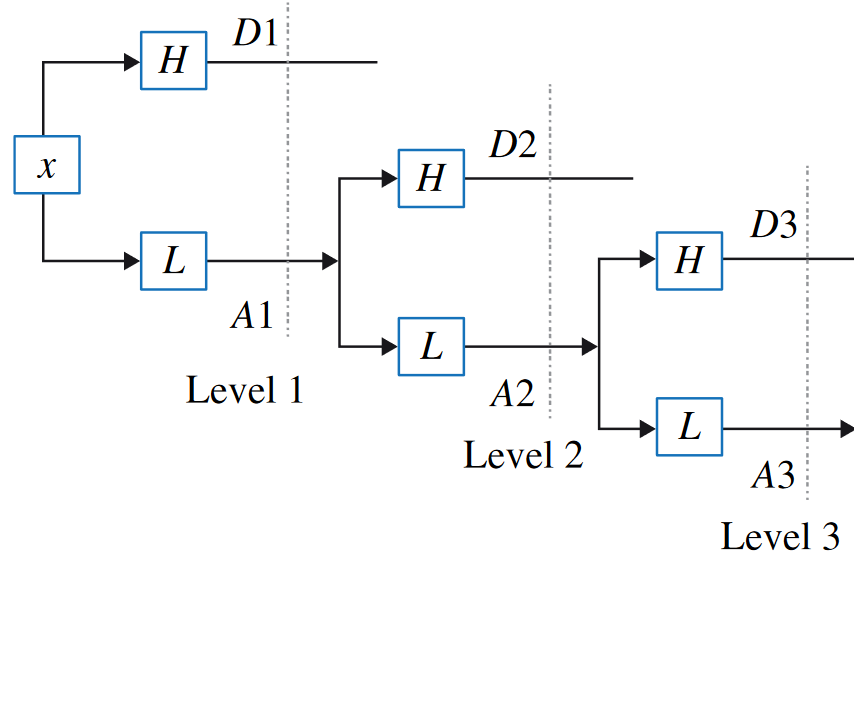
\includegraphics[width=\textwidth]{assets/analysis/DWT.png}
        \caption{Discrete wavelet transform}
        \label{fig:dwt-filter-bank}
    \end{subfigure}
    \hfill
    \begin{subfigure}[b]{0.49\textwidth}
        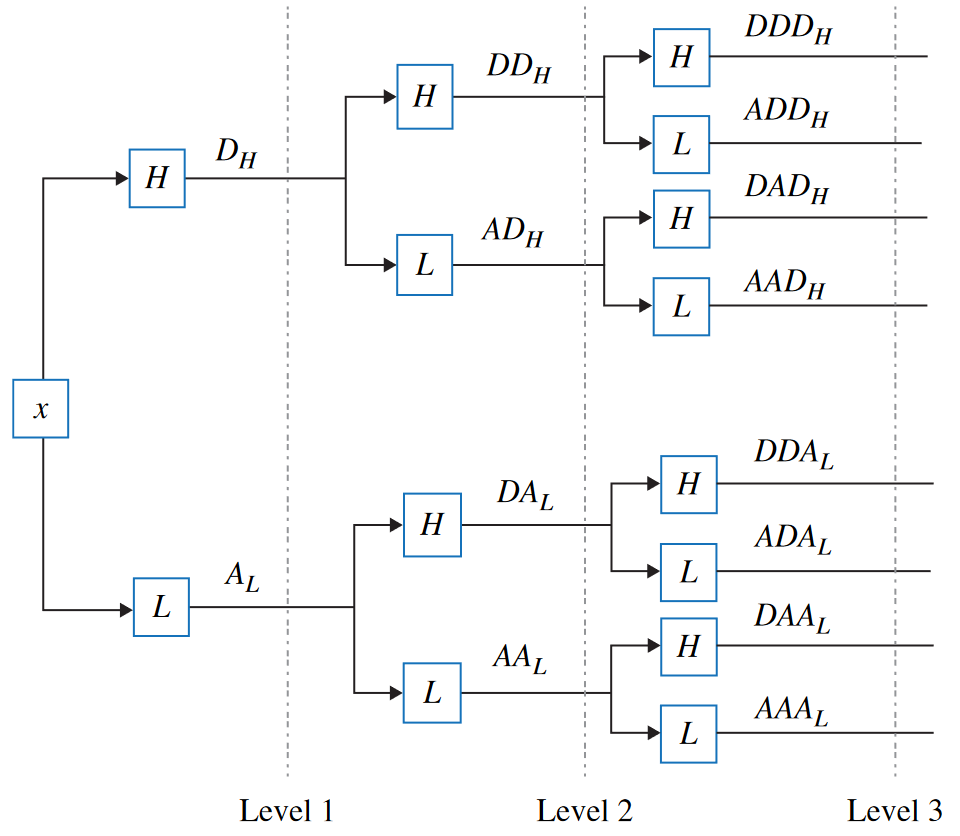
\includegraphics[width=\textwidth]{assets/analysis/WPD.png}
        \caption{Wavelet packet decomposition}
        \label{fig:wpd-filter-bank}
    \end{subfigure}
    \caption{Dyadic filter banks for discrete wavelet transform~\cite{nandi_condition_2019}}
\end{figure}

The wavelet packet energy ratio for weak feature extraction has been incorporated into the method of multiple frequency bands demodulation (MFBD). The highest $n$ energy coefficients are selected out of 8 narrow frequency bands to subsequently affect the principal components. Demodulation principle for the frequency bandwidth prescribes $n$ to satisfy condition: $1\;/\;2^n > f_{\mathrm{modulation}}\;/\;f_s$. The first few eigenvectors explaining together more than 80\% of energy are retained to reconstruct the signal with Fourier transform and retain the weak fault components~\cite{song_mfbd_2021}.

Tool wear diagnosis based on acoustic emission (AE) signal considers \emph{wavelet packet energy} in bands $E_{8}$, $E_{10}$, $E_{12}$, \emph{energy ratios} $P_{8}$, $P_{13}$, and \emph{energy entropy} as having high correlation ($|r| > 0.8$) with the band saw flank face width. The acoustic signal is decomposed into three layers using Daubechies db3 wavelet. The bottom layer contains bands numbered 7 through 14, each with a bandwidth of 62.5 kHz, because of the 1 MHz sampling frequency. The feature vector constructed in the article includes other statistical metrics out of power spectral density that has reached a notable correlation with evolving wear. The statistics are \emph{skewness}, \emph{kurtosis}, \emph{shape factor}, and \emph{centroid frequency}~\cite{zhuo_research_2022}.

Discrete wavelet transform and wavelet packets partition the spectrum into predefined frequency bands that do not always adequately capture individual elementary oscillations. Adaptive spectral segmentation is needed to extract separate intrinsic mode functions (IMF).

\subsection{Empirical wavelet features}
\textbf{Empirical Wavelet Transform} (EWT) constructs adaptive bandpass filters with Meyer wavelet. The inner product of the signal with the scaling function $\hat{\phi_n}$ obtains the approximation coefficients and the inner product with the wavelet function results in detail coefficients.

The normalized frequency axis in range $\omega \in [0, \pi]$ is divided by split points $\omega_0, \dots, \omega_N$ where $\omega_n = f_n \cdot 2 \pi\;/\;f_s$ (Fig.~\ref{fig:ewt-spectrum-segmentation}). Each segment is bounded between $[\omega_{n-1}, \omega_n]$ with transition phase of width $2\tau_n$ and polynomial transition function $\beta(x)$. A tight frame set of empirical wavelets is built by setting the transition phase proportional to the band boundary: $\tau_n = \lambda \omega_n$, and proportional constant must obey constrain: $\lambda = \min\left(\frac{\omega_{n+1} - \omega_n}{\omega_{n+1} + \omega_n}\right)$. The $N$ boundaries defining different portions of the Fourier spectrum are placed at the center between two consecutive local maxima~\cite{gilles_empirical_2013}.

\begin{figure}[ht]
    \centering
    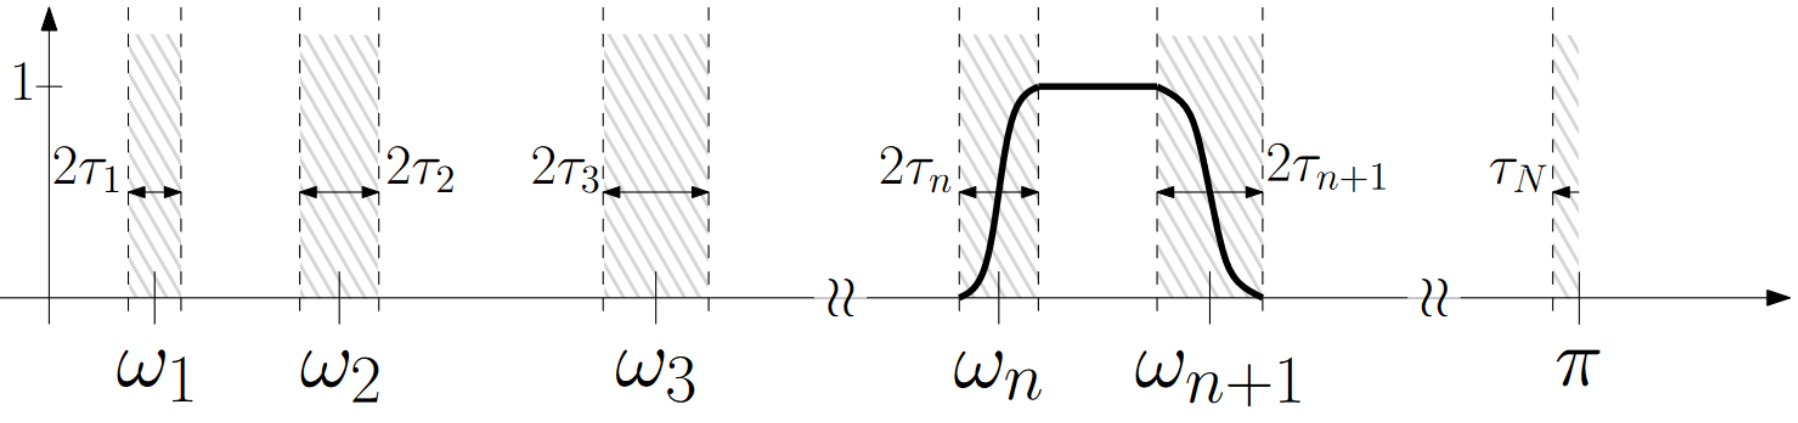
\includegraphics[width=0.9\textwidth]{assets/analysis/EWT.png}
    \caption{Empirical wavelet segmentation of Fourier spectrum~\cite{gilles_empirical_2013}}
    \label{fig:ewt-spectrum-segmentation}
\end{figure}

The drawback of EWT is improper segmentation in noisy and non-stationary signals producing too many uninformative partitions of the spectrum. The solutions we discuss fall into two groups that apply improvements before or after the wavelet transformation step. 

A combination of \textbf{Maximum Correlated Kurtosis Deconvolution} and improved EWT (MKCD-EWT) favors periodic impacts by dynamically constructing an optimal FIR filter that maximizes the correlation kurtosis of the signal. The envelope curve smooths of the amplitude spectrum by linear interpolation (Fig.~\ref{fig:mkcd-ewt-segmentation}). The threshold accounting for desired SNR modifies the envelope when more than $n$ components are discovered ($A_h$ is maximal amplitude and $A_l$ is minimal amplitude): $\lambda = A_l + \frac{C}{\mathrm{SNR}}(A_h - A_l)$. \emph{Squared envelope spectrum} and \emph{Teager energy operator spectrum} are computed as fault features for the IMF with highest kurtosis~\cite{li_fault_2019}. 

The segmentation boundaries detection can be accomplished also on the spectral envelope consisting of \textbf{Piecewise Cubic Hermite Interpolating Polynomial} (PCHIP-EWT) instead of scanning the Fourier spectrum directly (Fig.~\ref{fig:pchip-ewt-segmentation}). Divisions of the upper cut-off frequency are kept if local power indicates a subband with useful information ($p_i(f) \geq \lambda$)  as in the case of abrupt level change. Local power is the ratio of $n$th local envelope maximum and difference of indexes of its adjacent local minima:  $p_i(f) = K_{max(i)(f)} \;/\;\left(f_{k_{min(i+1)}} - f_{k_{min(i)}}\right)$. The best $\lambda$ is set experimentally~\cite{zhuang_improved_2020}.

\begin{figure}[ht]
    \centering
    \begin{subfigure}[b]{0.49\textwidth}
        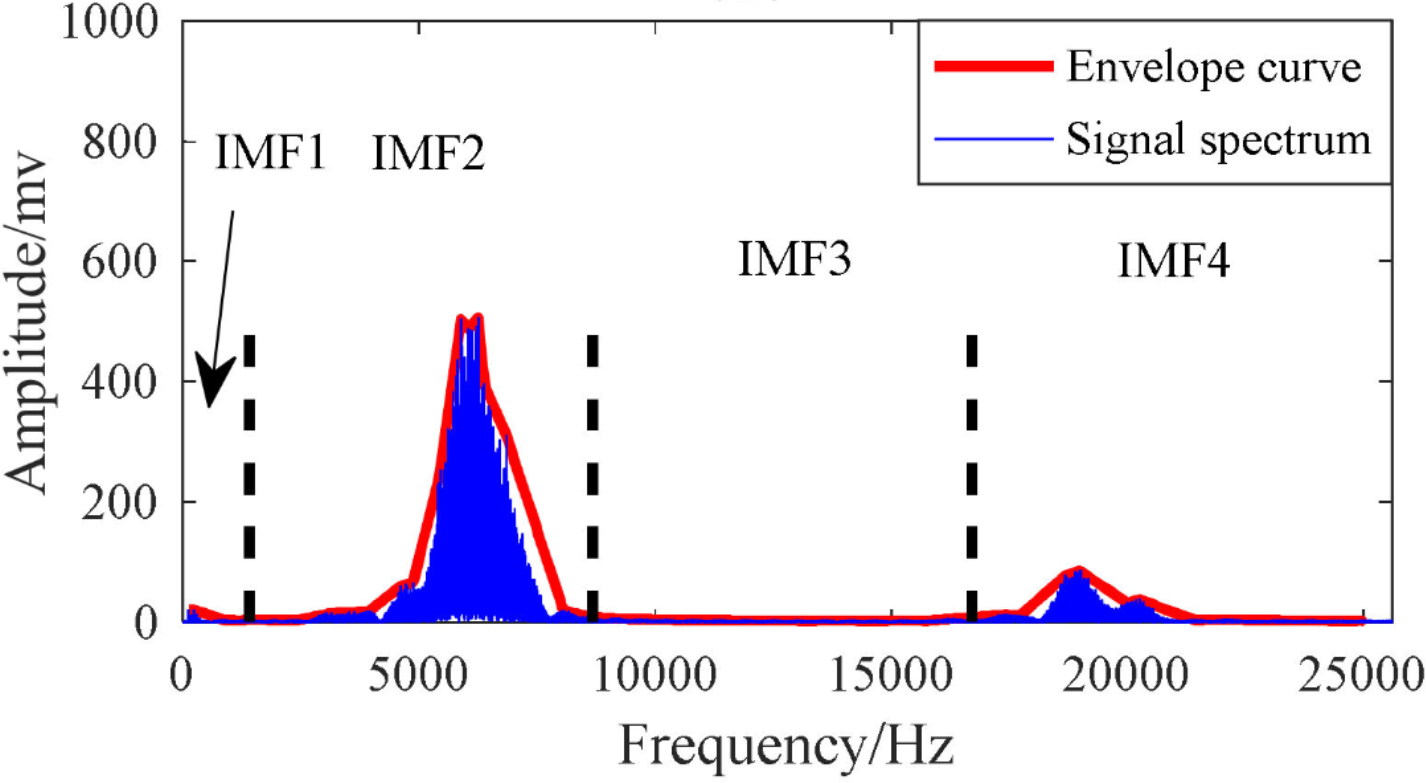
\includegraphics[width=\textwidth]{assets/analysis/MKCD-EWT.png}
        \caption{MKCD-EWT~\cite{li_fault_2019}}
        \label{fig:mkcd-ewt-segmentation}
    \end{subfigure}
    \hfill
    \begin{subfigure}[b]{0.49\textwidth}
        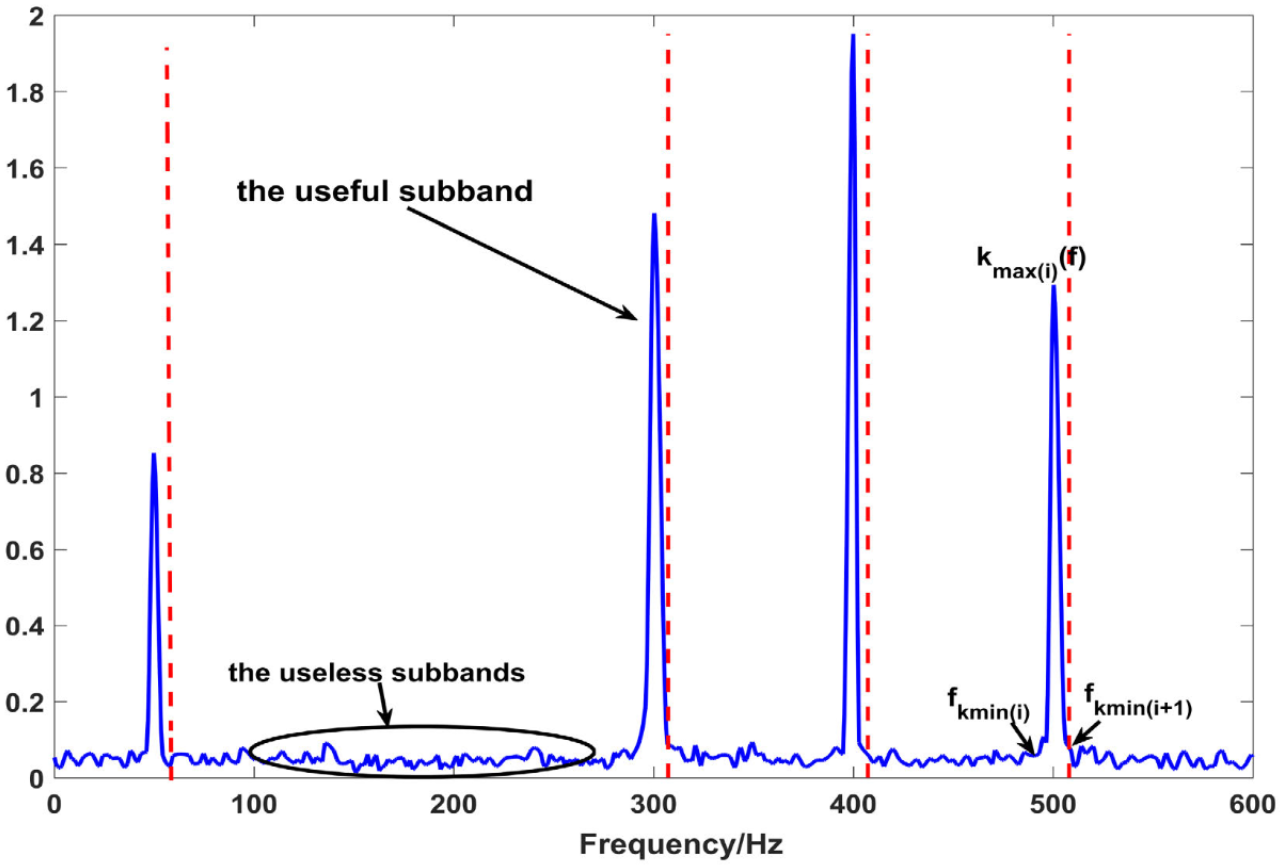
\includegraphics[width=\textwidth]{assets/analysis/PCHIP-EWT.png}
        \caption{PCHIP-EWT~\cite{zhuang_improved_2020}}
        \label{fig:pchip-ewt-segmentation}
    \end{subfigure}
    \caption{Illustration of improved EWT spectral segmentations}
\end{figure}

The inspiration for filtering with adaptive basis comes from \textbf{Empirical mode decomposition} (EMD). This procedure locates local maxima and minima in the time waveform that are interpolated with cubic splines to form signal envelopes. The average of the upper and lower envelope is repeatedly subtracted from the residuals recovering the higher order and lower frequency IMFs~\cite{wang_computational_2014}. 

The EMD is not recommended for practical applications because it suffers from mode mixing problems and lacks rigid theoretical foundations. Many improvements based on the mode sifting process, such as Local Mean Decomposition (LMD), Ensemble Empirical Mode Decomposition (EEMD), Concealed Component Decomposition (CCD)~\cite{tiwari_novel_2021}, and Empirical Wavelet Transform, have been devised as being capable of estimating more reasonable modes.

Wavelet domain features and associated spectral segmenation appears to be a powerful tool in conserving data bandwidth. For the use in white-box machinery diagnosis these trend indicator turn out to be difficult to comunicate and comprehend. Therefore we use more standardized metrics in the further study.

\section{Feature transformations}
Numerical features from the feature extraction phase have non-normal distributions and span the range of scales. Broad differences among features skew the spread in the particular axis. Inevitably it can degrade the discernment of fault diagnostics models that map input onto smooth function as regression does~\cite{zheng_feature_2018}. The feature scaling, power transform, and principal component analysis modify attribute values to gain more meaningful predictors, but one must be cautious in model interpretation.

\subsection{Feature normalization}
Vibrations are measured with an accelerometer in the form of 3D vectors where each axis has its component. Models have to be resilient to any slight inclination or sensor orientation. To satisfy this prerequisite, feature $f$ extracted from all three dimensions is first composed into a single vector and Euclidian norm is computed~\cite{kamminga_robust_2018}.

\myequations{Feature euclidian norm}
\begin{ceqn}\begin{align}
\widetilde{f} = \sqrt{f_x^2 + f_y^2 + f_z^2}
\label{equ:min-max-scaler}
\end{align}\end{ceqn}

Feature normalization most often takes two forms. \textbf{Min-max scaling} changes original range of values into interval $[0, 1]$ (Equation~\ref{equ:min-max-scaler}). \textbf{Standardization} (Equation~\ref{equ:standardization-scaler}) constrains the mean of the variable to 0 with a variance of 1~\cite{zheng_feature_2018}.

\myequations{Min-max feature scaling}
\begin{ceqn}\begin{align}
\widetilde{x} = \frac{x - \min(x)}{\max(x) - \min(x)}
\label{equ:min-max-scaler}
\end{align}\end{ceqn}

\myequations{Feature standardization}
\begin{ceqn}\begin{align}
\widetilde{x} = \frac{x - \bar{x}}{\sigma_x}
\label{equ:standardization-scaler}
\end{align}\end{ceqn}


\subsection{Principal components analysis}
Highly correlated features generated from a relatively small original column space are redundant as they do not provide any additional information for diagnostics. \textbf{Principal Component Analysis} (PCA) solves this problem by projecting potentially linearly dependant features into a new feature space where the incoming information is preserved in a smaller number of features~\cite{zheng_feature_2018}. The threshold of how many principal components are picked depends on the amount of explained variance and desired quantity of data reduction. 

\myequations{Singular Value Decomposition}
\begin{ceqn}\begin{align}
\mathbf{C} = \mathbf{U \Sigma V^T}
\label{equ:svd}
\end{align}\end{ceqn}

PCA consists of taking the Singular Value Decomposition (SVD) (Equation~\ref{equ:svd}) of the mean-centered input matrix. The disadvantage of this method is the loss of explainability in transformed space though it generally outperforms the model working with hand-crafted features~\cite{brito_fault_2021}. The signal samples can be processed directly by PCA without going through an intermediate step of calculating statistical measures. 

\section{Feature selection}
Features do not contribute to predictive power of the model with an even share. A certain subset can reach better results than others. Choosing optimal feature subset is NP-hard combinatorial problem.

\subsection{Filtering methods}
The features can be chosen intrinsically as a part of a model by \emph{embedded methods} or by machine learning search algorithm at a serious computational expense in \emph{wrapper methods}. However, we will focus on \emph{filtering methods} which rank the predictors in order of their importance for the problem at hand and separate the best performing group~\cite{johnson_feature_2019}. The most common strategy is \emph{K-Best Selection}.

The general steps in selecting the adequate predictors is as follows~\cite{nandi_condition_2019}:
\begin{enumerate}
    \itemsep0pt
    \item \textbf{Subset generation} - sets of features are generated in different search directions and with various strategies. Attributes are either appended to an empty set or pruned away from a universal set, sequentially or randomly.
    \item \textbf{Subset evaluation} - comparison of subset quality is assessed with relevance measure some of which are discussed below.
    \item \textbf{Stopping criteria} - search is exhausted when the specified number of features has been found, subset metrics cannot be improved further, or satisfactory model performance is achieved. Subset generation and evaluation can be performed multiple times until the stopping criteria are met.
    \item \textbf{Validation} - resulting subset is tested for the specific model on synthetic and real-world datasets against well-known results. 
\end{enumerate}

Filter-based feature selection is preprocessing step independent of model choice with small computational requirements. Measures of information, correlation, similarity, and interdependence output the relevancy rating. Predictors are rated individually or in interacting congregations. 

\subsection{Scores for ranking}
Most of the scores are based on supervised learning, so they expect true class labels to apportion the measurements respectively. After the scores are assigned to the first $n$ features, those below a threshold are removed. 

The frequently used scores upon which the feature relevance is ordered are~\cite{nandi_condition_2019}: 
\begin{itemize}
\item \textbf{Variance threshold} - removes low-variance features below set threshold.
\item \textbf{Correlation coefficient} - expresses the linear relationship between two variables. The codependent variables are of three sorts: quantitative, ordinal, and nominal. The choice of coefficient calculation is determined by the type of variables under consideration shown in Table \ref{tab:corr-coef}. 

\emph{Pearson correlation} coeficient expresses similarity between two quantitative features $f_i$ and $f_j$. In the classification setting the correlation of feature $f$ makes sense only with dichotomous target class label $c$ using \emph{point biserial coeficient}. Mathematically, this is equivalent to the Pearson coefficient. Rank correspondence is quantified with either Spearman rho or Kendall's Tau~\cite{calkins_more_2005}.

\begin{table}[ht]
\renewcommand{\arraystretch}{1.5}
\begin{adjustbox}{width=\columnwidth,center}
\begin{tabular}{|c|l|l|l|}
\hline
\textbf{Variable Y\textbackslash{}X} & \multicolumn{1}{c|}{\textbf{Quantitiative X}} & \multicolumn{1}{c|}{\textbf{Ordinal X}} & \multicolumn{1}{c|}{\textbf{Nominal X}} \\ \hline
\textbf{Quantitative Y}              & Pearson $r$                                   & Biserial $r_b$                          & Point Biserial $r_{pb}$                 \\ \hline
\textbf{Ordinal Y}                   & Biserial $r_b$                                & Spearman $\rho$    & Rank Biserial $r_{rb}$                  \\ \hline
\textbf{Nominal Y}                   & Point Biserial $r_{pb}$                       & Rank Bisereal $r_{rb}$                  & Phi, L, C, Lambda                       \\ \hline
\end{tabular}
\end{adjustbox}
\caption{Correlation coeficients}
\label{tab:corr-coef}
\end{table}

Attributes are ranked in descending order according to the absolute value of their correlation coefficient. We seek the highest correlation to the class label.
\myequations{Pearson correlation coefficient}
\begin{ceqn}\begin{align}
r(i) = \frac{\mathrm{cov}(f, c)}{\sqrt{\mathrm{var}(f) \cdot \mathrm{var}(c)}}
\end{align}\end{ceqn}

\item \textbf{Fisher score} - measures the difference among the means of the classes. It is interchangeable with ANOVA F-value, but it is evaluated for each feature $X^j$ separately. Ideally, the features in the subset have large distances between samples of various classes in $C$ and distances within a class are the smallest possible. In the formula (\ref{equ:fisher-score}), $n_j$ is the sample size of $j$th feature, $\mu^j$ is its sample mean, and $\mu$ is the overall mean.

\myequations{Fisher score}
\begin{ceqn}\begin{align}
\mathrm{FS}(X^j) = \frac{\sum_{i=1}^{C} n_i(\mu_i^j - \mu^i)^2}{\sum_{i=1}^{C} (n_i - 1) \cdot (\sigma_i^j)^2}
\label{equ:fisher-score}
\end{align}\end{ceqn}

\item \textbf{Mutal information} - quantifies the dependence among features, or between features and class labels. It is almost identical to Information Gain. The probability distribution proximity of variables derives from relative entropy known as the Kullback-Leibler distance. Mutual information presumes variables are discrete. In the case of quantitative variables, mutual information is estimated with binning or nearest neighbors methods~\cite{ross_mutual_2014}.

Probabilities $P(x)$, $P(y)$, $P(x, y)$ are estimated in the contingency table from event occurrence count to all sample population $|x|\;/\;N$. Joint probability $P(x, y)$ represents samples of feature $x$ simultaneously in class $y$.

\myequations{Mutal information}
\begin{ceqn}\begin{align}
\mathrm{MI}(X, Y) = \sum_{y \in Y} \sum_{x \in X} P(x, y) \cdot \log\left(\frac{P(x, y)}{P(x)P(y)}\right)
\end{align}\end{ceqn}
\end{itemize}

Multiple subsets of predictors produced by each evaluation metric can train several variants of a classification model. Sets of attributes can be combined into an ensemble by \emph{electoral system}. One such example is \textbf{majority voting} which chooses the best feature out of the group. \textbf{Rank product} unifies several feature orderings by computing the geometric mean of feature rank in every experiment realization~\cite{breitling_rank_2004}.